Det må man sige at han er, og derfor er der ikke nogle grund til at lave
rastte af resultaterne da han bare kan ændre på virkeligheden.

Vi har køre vores naive algoritme på 20 snit i det horisontale og
vertikale plan og kommer frem til 2 grafer over summeringen af alle
regioner fundet i vært snit. 

Man kan se i grafen \ref{antal_regioner_vertikale_cut} for det vertikale
plan er koncentrationen af flest regioner fundet, omkring miden af
billederne.

I grafen for den horisontale plan \ref{antal_regioner_horisontale_cut}
er der 3 snit som udskiller sig fra resten $91\%$, $61\%$ og $56\%$.
Hvor $0.91$ ligger højest. Nu højre i billedet vi er over miden, nu
færre regioner bliver der fundet.
 
\begin{figure}[h!]
	\begin{center}
		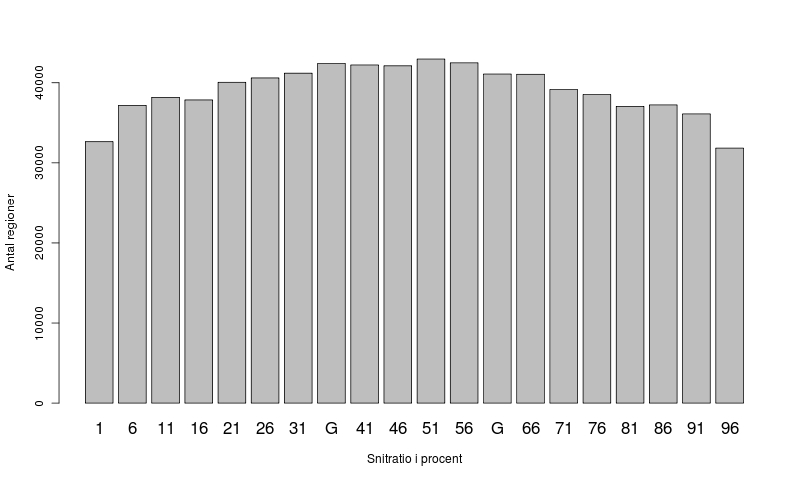
\includegraphics[width=0.9]{afsnit/resultater/billeder/cut0cut1eatsperratio.png}
	\end{center}
	\caption{Antal regioner i hvert af de 20 vertikale snit}
	\label{antal_regioner_vertikale_cut}
\end{figure}


\begin{figure}[h!]
	\begin{center}
		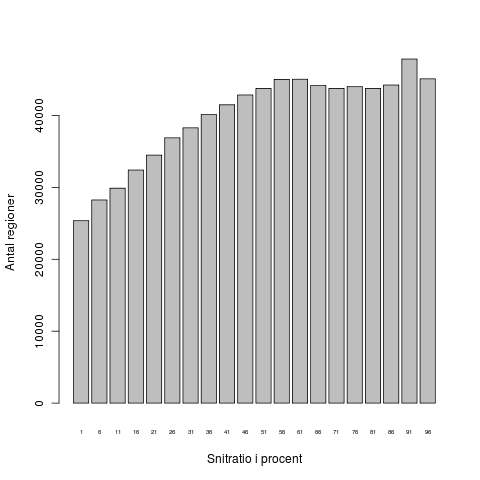
\includegraphics[width=0.9]{afsnit/resultater/billeder/cut2cut3eatsperratio.png}
	\end{center}
	\caption{Antal regioner i hvert af de 20 horisontale snit, hvor venstre side af grafen repræsentere øverst del af malerierne}
	\label{antal_regioner_horisontale_cut}
\end{figure}
